\chapter{Implementacija}
\label{chp:Implementation}

U ovom poglavlju će biti opisana implementacija pratećeg projekta pisanog u programskom jeziku C\# 8.0, koristeći \emph{.NET Core 3.1} radni okvir. C\# je izabran zbog lakoće implementacije velikih projekata i velike podrške paketa koji se mogu preuzeti, od kojih su korišćeni \emph{ANTLR Runtime} paket koji daje potrebne biblioteke za rad sa ANTLR generisanim parserima i \emph{Math.NET Symbolics} paket za rad sa simboličkim vrednostima. Rezultat je konzolna aplikacija koja može da generiše, serijalizuje ili prikaže opšti AST za dati izvorni kod, ali i da poredi takav AST sa drugim. Čitav projekat je dostupan u potpunosti na servisu GitHub na adresi \url{https://github.com/ivan-ristovic/LICC}.

Jedan od glavnih ciljeva aplikacije je modularnost i jednostavna proširivost. U tom duhu se, pored implementacije klasa potrebnih za predstavljanje opšte AST apstrakcije, pruža i interfejs za kreiranje adaptera koji će od proizvoljnog stabla parsiranja kreirati opšti AST. Kao primer, adapteri su kreirani za programske jezike C i Lua, a za primer potpune slobode u izboru gramatike je kreirana gramatika za pseudo-jezik i adapter za istu, što dozvoljava poređenje kodova sa specifikacijom datom u obliku pseudo-koda. Čitav projekat se sastoji od više komponenti, od kojih su značajnije:
\begin{itemize}
    \item Biblioteka koja pruža klase za rad sa opštom AST apstrakcijom
    \item Komponenta za kreiranje AST od proizvoljne gramatike putem adaptera --- moguća serijalizacija u JSON
    \item Komponenta za semantičko poređenje opštih AST --- konzolni izlaz
    \item Komponenta za AST vizualizaciju --- grafički prikaz AST
    \item Korisnički interfejs --- komandna linija
\end{itemize}

Čitava arhitektura data putem UML dijagrama komponenti se može videti na slici \ref{fig:ImplementationComponents}. Osim implementacije same aplikacije, svaki funkcionalni deo projekta prate i testovi jedinica koda, koji su povezani sa \emph{GitHub Actions} porškom za neprekidnu integraciju.

\begin{figure}[h!]
\centering
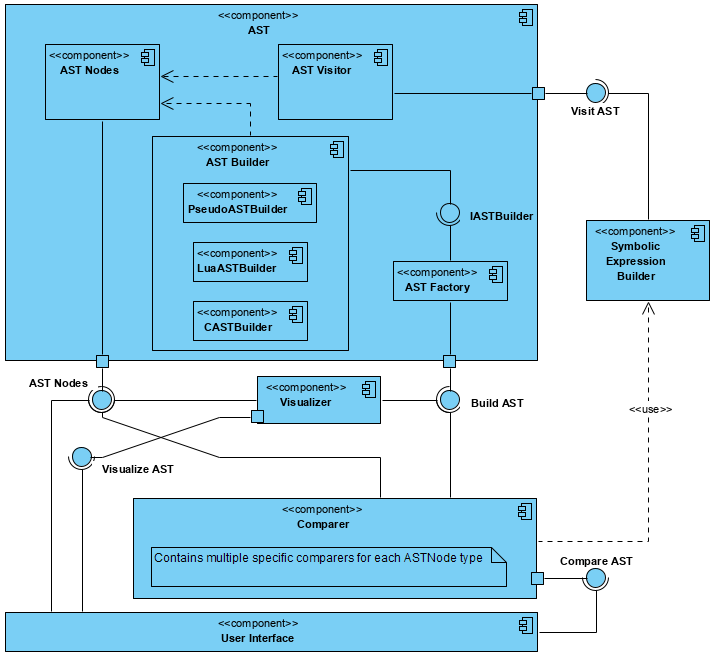
\includegraphics[scale=0.8]{images/uml/ComponentDiagram.png}
\caption{UML dijagram komponenti implementacije.}
\label{fig:ImplementationComponents}
\end{figure}


\section{Implementacija apstrakcije}
\label{sec:ImplementationMyAST}

Implementacija prati hijerarhije opisane u poglavlju \ref{chp:MyAST} kroz mehanizam nasleđivanja. Svaki tip čvora je implementiran kao zasebna klasa koja nasleđuje apstraktnu klasu \texttt{ASTNode}. Dijagram klasa koje nasleđuju klasu \texttt{ASTNode} se može videti na slikama \ref{fig:UMLASTNode1} i \ref{fig:UMLASTNode2}. Pored implementacije klasa koje predstavljaju AST čvorove, kreiran je i javno dostupni interfejs za obilazak AST putem obrazca posetilac u implementaciji korišćen za kreiranja graditelja simboličkog izraza od AST koji predstavlja izraz kao i evaluatora takvog AST.

\begin{figure}[h!]
\centering
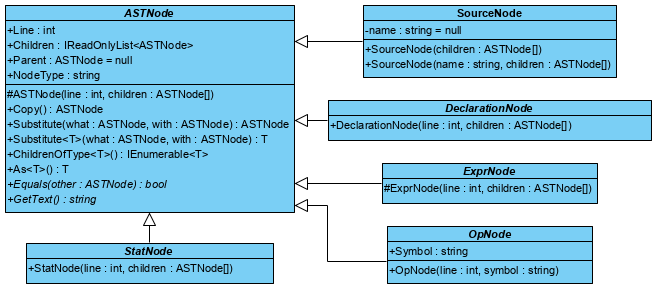
\includegraphics[scale=0.7]{images/uml/ASTNode.png}
\line(1,0){450}\\
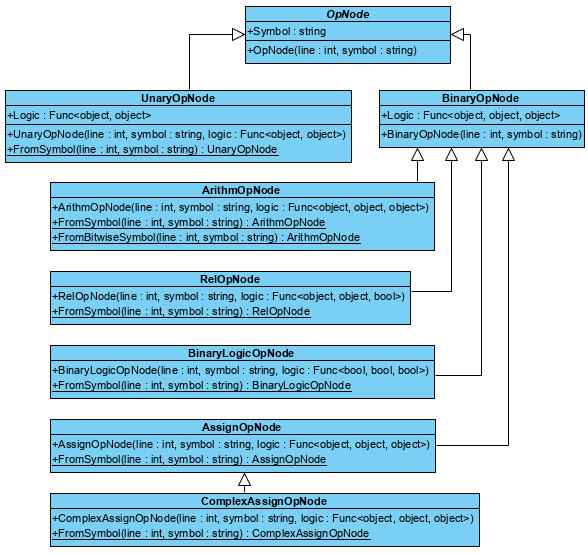
\includegraphics[scale=0.7]{images/uml/OperatorNode.png}
\caption{UML klasni dijagram (deo 1).}
\label{fig:UMLASTNode1}
\end{figure}

\begin{figure}[h!]
\centering
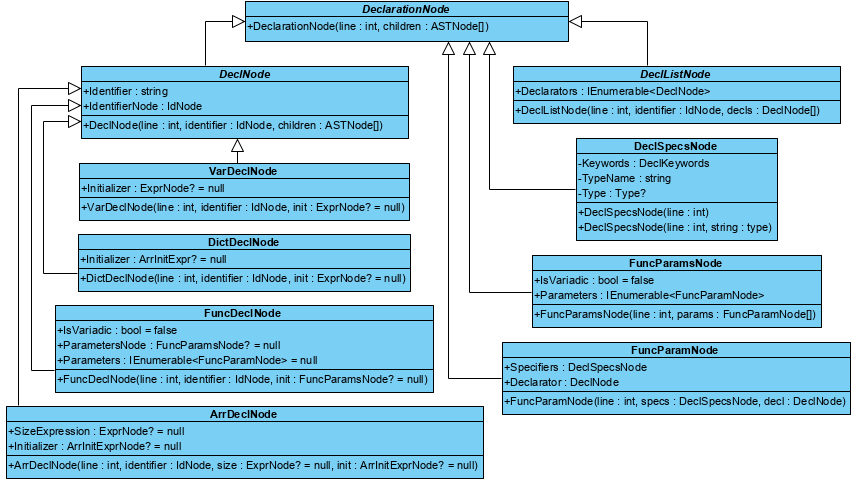
\includegraphics[scale=0.65]{images/uml/DeclarationNode.png}
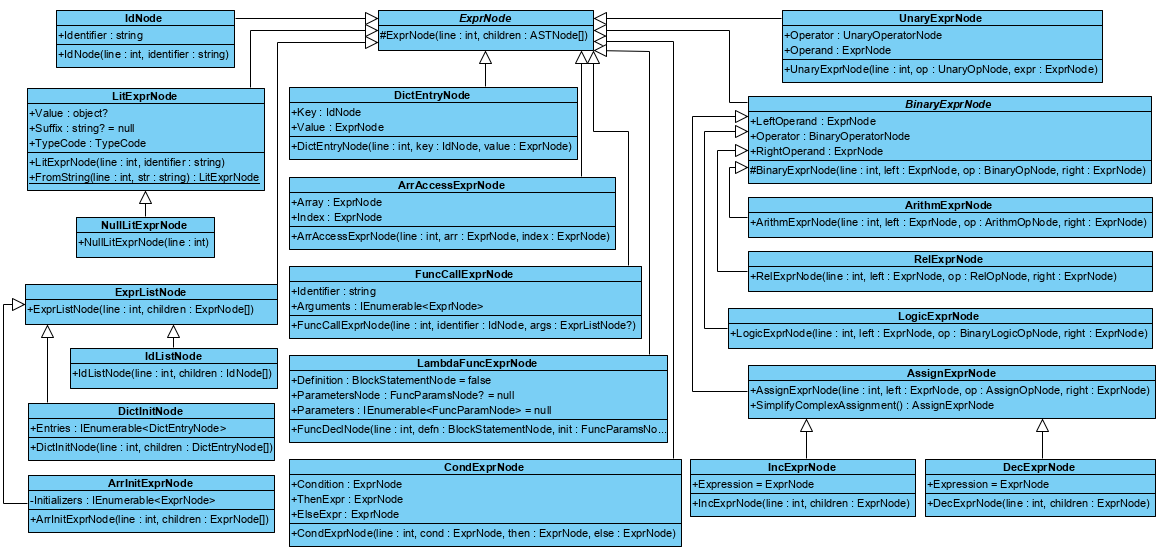
\includegraphics[scale=0.55]{images/uml/ExpressionNode.png}
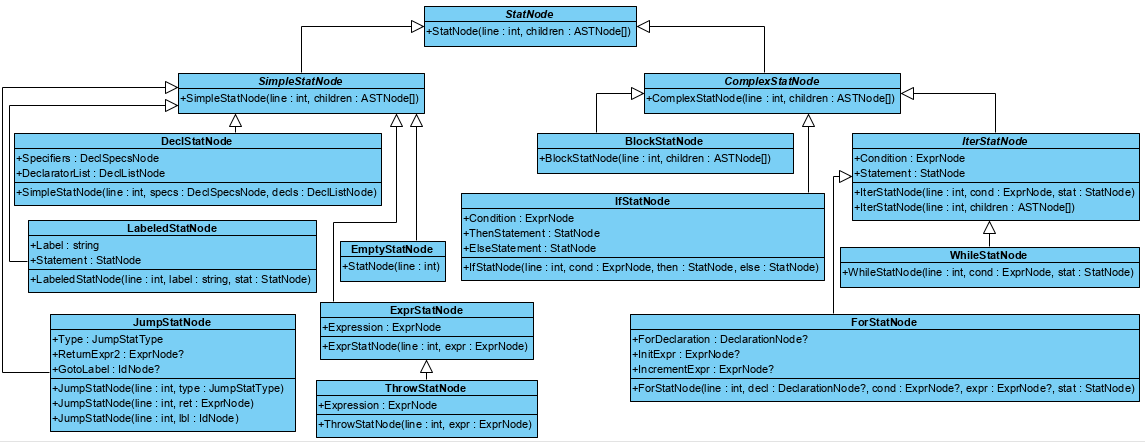
\includegraphics[scale=0.55]{images/uml/StatementNode.png}
\caption{UML klasni dijagram (deo 2).}
\label{fig:UMLASTNode2}
\end{figure}

AST struktura je \emph{imutabilna} --- ne mogu se dodavati ili uklanjati deca čvorovima. Moguće je klonirati AST čvorove ili vršiti zamenu određenog podstabla drugim podstablom ne menjajući original. Svaki AST čvor se može porediti po jednakosti sa drugim AST čvorom po intuitivnoj logici poređenja pruženom kroz predefinisane operatore poređenja.

\section{implementacija upoređivača}
\label{sec:ImplementationComparer}

\pangrami
\section{Implementacija vizualnog prikaza AST}
\label{sec:ImplementationVisualizer}


\section{Implementacija korisničkog interfejsa}
\label{sec:ImplementationUI}


